

\section*{Introduction}

In previous lesson, we solved linear inequalities. 
Our solutions to those problems generally came in two parts:
\begin{itemize}
    \item an inequality with the variable (for example, $x \geq 5$), and
    \item a graph of that inequality on the number line (which involves circled and arrows).
\end{itemize}

\myEmptyExampleBox[4in]{0.75in}{
    \small\itshape
    For example, the solution to $2x+5 \leq 25$ would look like this.
}


In this lesson we will be working with more complicated inequalities called
{\bfseries\itshape compound inequalities}.
Their solutions will also come in two parts (inequalities and number lines).
But since the problems are more complicated, the inequalities and number lines will also be more complicated.



\section*{Graphing inequalities connected by ``and''}

\begin{myExample}{
    The graph {\sffamily\bfseries A} shown below is for the inequality 
    \[x \geq -1\]
    Which of the values of $x$ shown in the table are allowed by this graph?
}
    \begin{center}
        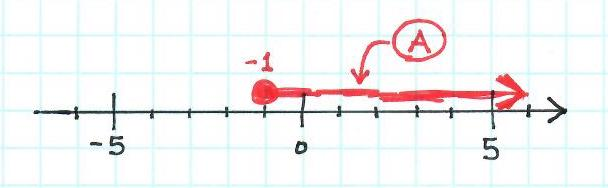
\includegraphics[width=3in]{and-1.jpg}
        
        \Large
        \begin{tabular}{c|c}
            $x$ & yes or no? \\
            \toprule
            -2 & \\
            -1& \\
            0& \\
            1& \\
            2& \\
            3& \\
            4& \\
            \bottomrule
        \end{tabular}
    \end{center}
\end{myExample}


\begin{myExample}{
    The graph {\sffamily\bfseries B} shown below is for the inequality 
    \[x < 3\]
    Which of the values of $x$ shown in the table are allowed by this graph?
}
    \begin{center}
        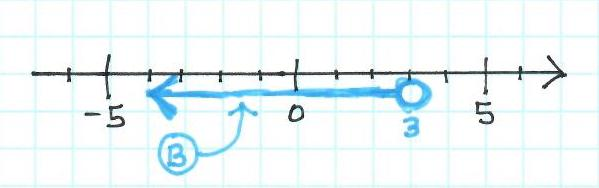
\includegraphics[width=3in]{and-2.jpg}
        
        \Large
        \begin{tabular}{c|c}
            $x$ & yes or no? \\
            \toprule
            0& \\
            1& \\
            2& \\
            3& \\
            4& \\
            \bottomrule
        \end{tabular}
    \end{center}
\end{myExample}


\begin{myExample}{
    Which of the values of $x$ shown in the table are allowed by 
    both graphs {\sffamily\bfseries A} and {\sffamily\bfseries B} at the same time?
}
    \begin{center}
        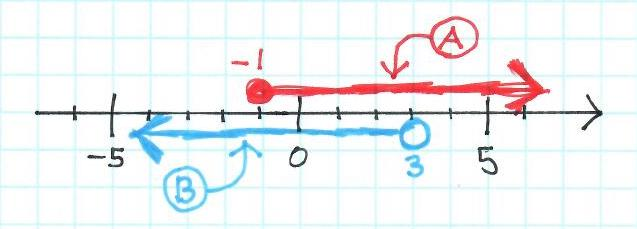
\includegraphics[width=3in]{and-3.jpg}
        
        \Large
        \begin{tabular}{c|c}
            $x$ & yes or no? \\
            \toprule
            -2 & \\
            -1& \\
            0& \\
            1& \\
            2& \\
            3& \\
            4& \\
            \bottomrule
        \end{tabular}
    \end{center}
\end{myExample}



\begin{myExample}{
    The ``overlap'' of 
    both graphs {\sffamily\bfseries A} and {\sffamily\bfseries B} 
    is the graph of this {\bfseries\itshape compound inequality} connected by ``and'':
    \[
        x \geq -1 \qquad \text{\itshape AND} \qquad x < 3
    \]
}
    \begin{center}
        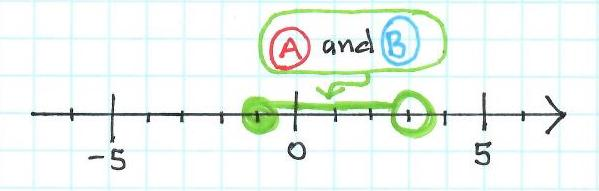
\includegraphics[width=3in]{and-4.jpg}
    \end{center}
\end{myExample}

\begin{center}
\begin{tcolorbox}[width=5.5in]
    To sketch the graph of two inequalities connected by ``and'',
    sketch the {\bfseries\itshape intersection} (``overlap'') of the graphs of each inequality.
\end{tcolorbox}
\end{center}








\section*{Graphing inequalities connected by ``or''}


\begin{myExample}{
    The graph {\sffamily\bfseries C} shown below is for the inequality 
    \[
        x > 2
    \]
    Which of the values of $x$ shown in the table are allowed by this graph?
}
    \begin{center}
        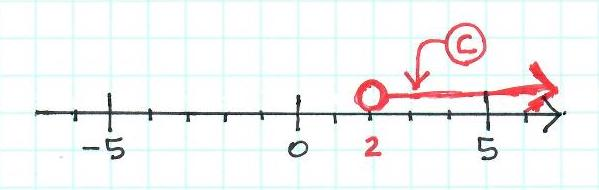
\includegraphics[width=3in]{or-1.jpg}
        
        \Large
        \begin{tabular}{c|c}
            $x$ & yes or no? \\
            \toprule
            0& \\
            1& \\
            2& \\
            3& \\
            4& \\
            5& \\
            \bottomrule
        \end{tabular}
    \end{center}
\end{myExample}



\begin{myExample}{
    The graph {\sffamily\bfseries D} shown below is for the inequality 
    \[
        x \leq -3
    \]
    Which of the values of $x$ shown in the table are allowed by this graph?
}
    \begin{center}
        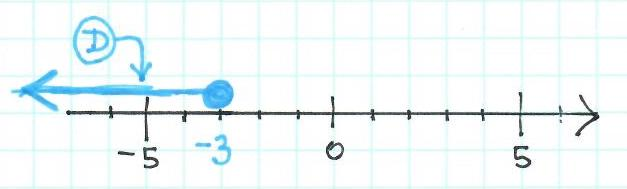
\includegraphics[width=3in]{or-2.jpg}
        
        \Large
        \begin{tabular}{c|c}
            $x$ & yes or no? \\
            \toprule
            -4& \\
            -3& \\
            -2& \\
            -1& \\
            0& \\
            \bottomrule
        \end{tabular}
    \end{center}
\end{myExample}



\begin{myExample}{
    Which of the values of $x$ shown in the table are allowed by 
    either graph {\sffamily\bfseries C} or {\sffamily\bfseries D}?
}
    \begin{center}
        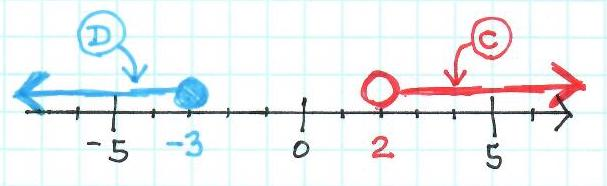
\includegraphics[width=3in]{or-3.jpg}
        
        \Large
        \begin{tabular}{c|c}
            $x$ & yes or no? \\
            \toprule
            -4& \\
            -3& \\
            -2& \\
            -1& \\
            0& \\
            1& \\
            2& \\
            3& \\
            4& \\
            5& \\
            \bottomrule
        \end{tabular}
    \end{center}
\end{myExample}



\begin{myExample}{
    The ``combination'' of graph {\sffamily\bfseries C} and graph {\sffamily\bfseries D} 
    is the graph of this {\bfseries\itshape compound inequality} connected by ``or'':
    \[
        x > 2 \qquad \text{\itshape OR} \qquad x \leq -3
    \]
}
    \begin{center}
        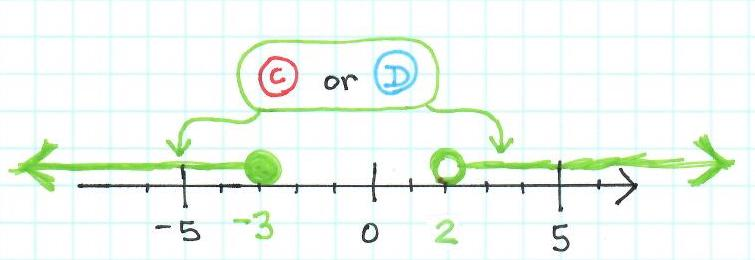
\includegraphics[width=3in]{or-4.jpg}
    \end{center}
\end{myExample}

\begin{center}
\begin{tcolorbox}[width=5.5in]
    To sketch the graph of two inequalities connected by ``or'',
    sketch the {\bfseries\itshape union} (``combination'') of the graphs of each inequality.
\end{tcolorbox}
\end{center}